
\documentclass[fleqn,addpoints]{exam}

\usepackage{graphicx}
\usepackage{booktabs}
\usepackage{float}
\usepackage{amsmath}
\usepackage{cancel}
\usepackage{polynom}
\usepackage{caption}
\usepackage{mdwlist}

\newcommand{\degree}{\ensuremath{^\circ}} 

\printanswers

\ifprintanswers 
\usepackage{2in1, lscape} 
\fi

\title{Math 115 \\ Homework 28}
\date{June 28, 2011}

\begin{document}

\maketitle

% \begin{figure}[H]
%   \centering
%   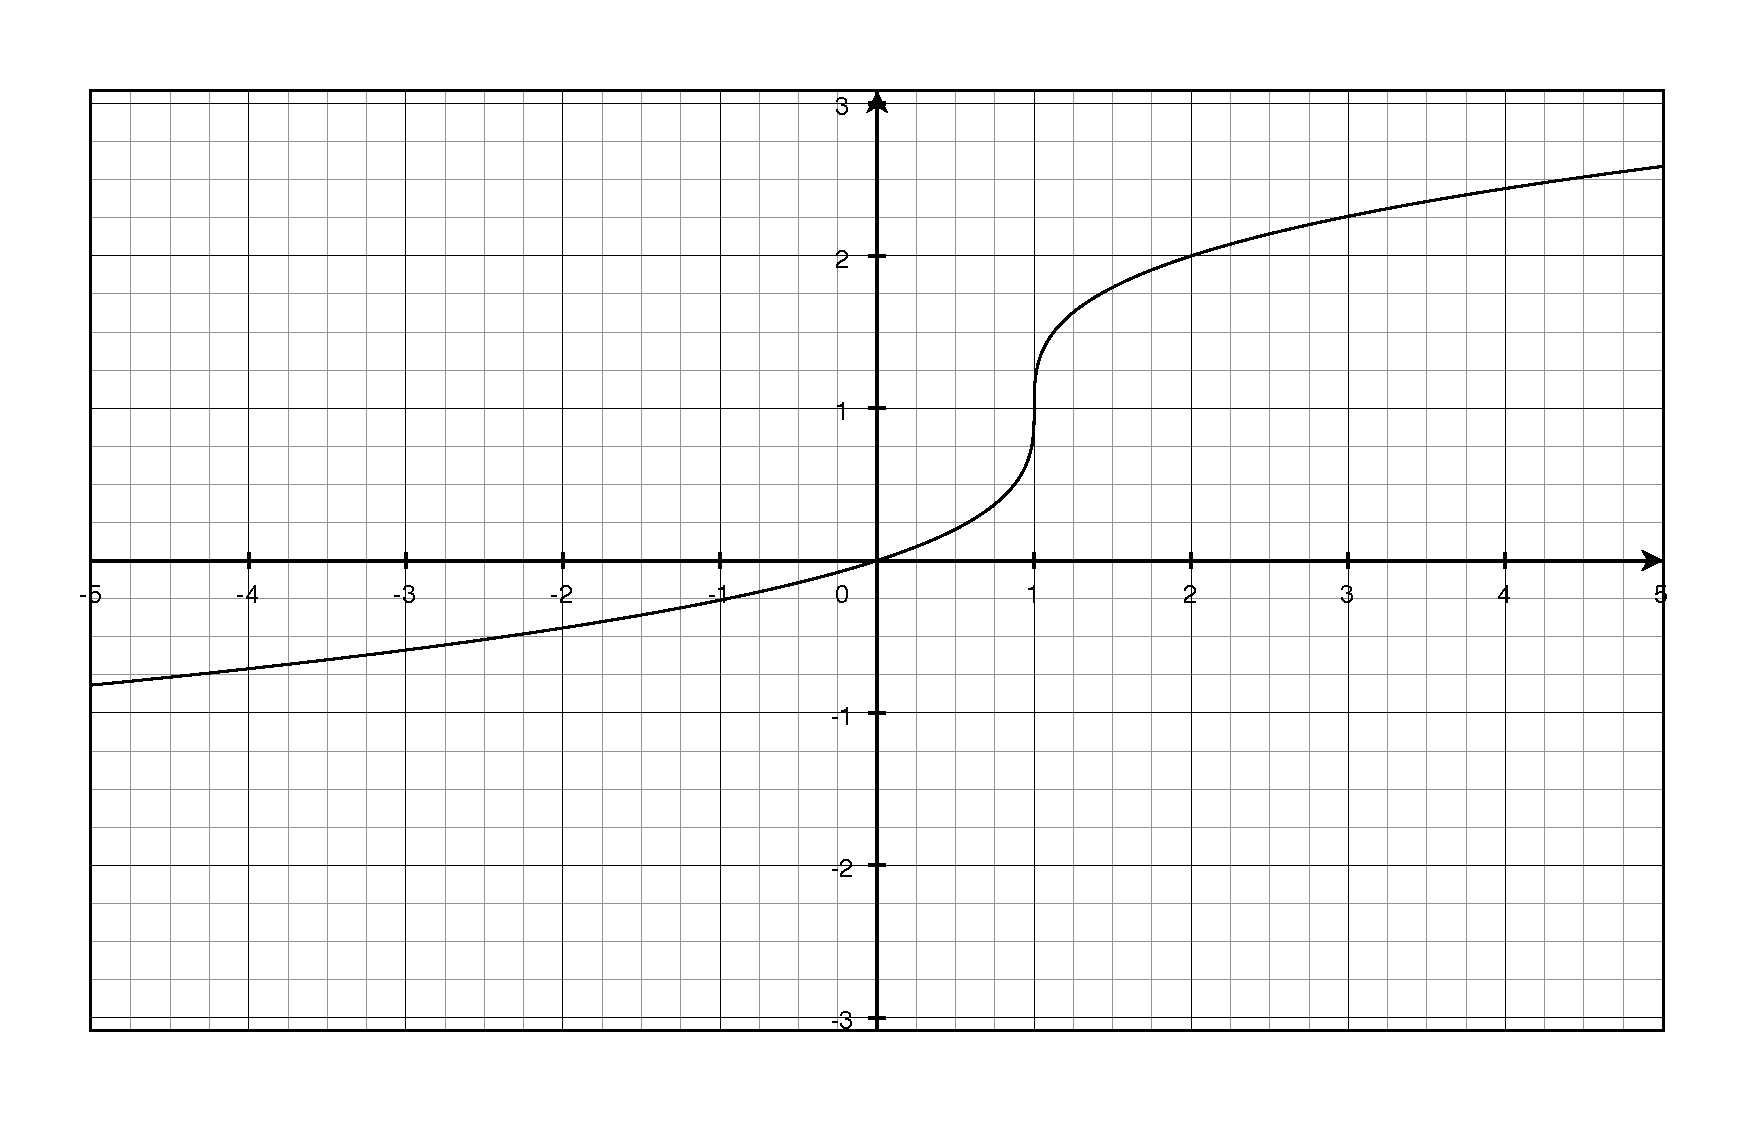
\includegraphics[scale=.3]{question7.eps}
%   \caption*{Question 7}
% \end{figure}

% \begin{tabular}{cc}
% \toprule
% period & amplitude \\
% \midrule
%   $\pi$ & $2$ \\
% \bottomrule
% \end{tabular}

\section{Homework}
\begin{itemize*}
  \item pp. 464-467: 7, 12, 15-16, 19-20, 23-24, 27-28, 30-31, 33-34, 57-58, 61-62, 68, 72,  77-78
  \item pp. 782-785: 5-10, 11-12, 17-18, 23-24, 31, 34, 37, 47, 50, 61, 68-69
\end{itemize*}

\section{Extra Credit}
Page 784, question 65

\ifprintanswers

\begin{description}
\item[a] $v = 17500 \cdot \sqrt{2} \approx = 24749 \text{ mph}$

\item[b]
The distance from the focus to the vertex is 4,100 miles, so this is $p$.

If you put the vertex at the origin and use the diagram, the equation is:
\begin{align*}
  x^2 &= -4 \cdot 4100 y \\
  x^2 &= -16400 y \\
\end{align*}

The answer in the back of the book puts the center of the earth at the origin, which puts the vertex at $(0, 4100)$:

\[
  x^2 = -16400(y - 4100)
\]

\end{description}

\begin{description}

\section{Pages 464-467}

\item[7] 
\begin{align*}
  2 \cos x + 1 &= 0 \\  
  2 \cos x &= -1 \\  
  \cos x  &= - \frac{1}{2} \\  
  x &= \left\{ \frac{2 \pi}{3} + 2n \pi, \frac{4 \pi}{3} + 2n \pi \right\} \\
\end{align*}

\item[12] 
\begin{align*}
  3 \cot^2 x - 1 &= 0 \\    
  3 \cot^2 x &= 1 \\  
  \cot x &= \pm \frac{\sqrt{3}}{3} \\  
  x &= \left\{ \frac{\pi}{3} + n \pi, \frac{2 \pi}{3} + n \pi \right\} \\
\end{align*}

\item[15] 
\begin{align*}
  4 \cos^2 x - 1 &= 0 \\  
  \cos^2 x &= \frac{1}{4} \\  
  \cos x &= \pm \frac{1}{2} \\  
  x &= \left\{ \frac{\pi}{3} + 2n \pi, \frac{2 \pi}{3} + 2n \pi \right\} \\
\end{align*}

\item[16] 
\begin{align*}
  \sin^2 x &= 3 \cos^2 x \\  
  1 - \cos^2 x &= 3 \cos^2 x \\  
  4 \cos^2 x &= 1 \\  
  \cos x &= \pm \frac{1}{2} \\  
  x &= \left\{ \frac{\pi}{3} + 2n \pi, \frac{2 \pi}{3} + 2n \pi \right\} \\
\end{align*}

\item[19] 
\begin{align*}
  \tan 3x ( \tan x - 1) = 0 \\ 
  \tan 3x = 0 \text{ or } \tan x - 1 = 0 \\
\end{align*}

If $\tan 3x = 0$:
\begin{align*}
  3x &= 0, \pi, 2\pi, 3\pi, \ldots \\
  x &= 0, \frac{\pi}{3}, \frac{2\pi}{3}, \frac{3\pi}{3}, \ldots \\
  x &= \frac{n \pi}{3} \\
\end{align*}

If $\tan x = 1$, $x = \dfrac{\pi}{4} + n \pi$.

So the answer is: $x = \left\{ \dfrac{n \pi}{3}, \dfrac{\pi}{4} + n \pi \right\}$.

\item[20] 
\begin{align*}
  \cos 2x ( 2 \cos x + 1) = 0 \\ 
  \cos 2x = 0 \text{ or } 2 \cos x + 1 = 0 \\
\end{align*}

If $\cos 2x = 0$:
\begin{align*}
  2x &= \frac{\pi}{2}, \frac{3 \pi}{2}, \frac{5 \pi}{2}, \ldots \\
  x &= \frac{\pi}{4}, \frac{3 \pi}{4}, \frac{5 \pi}{4}, \ldots \\
  x &= \frac{\pi}{4} + \frac{n \pi}{2} \\
\end{align*}

So the answer is: $x = \left\{ \dfrac{\pi}{4} + \dfrac{n \pi}{2}, \dfrac{2 \pi}{3} + 2n\pi, \dfrac{4 \pi}{3} + 2n \pi \right\}$.

\item[23] 
\begin{align*}
  3 \tan^3 x = \tan x \\ 
  3 \tan^3 x - \tan x = 0 \\ 
  \tan x ( 3 \tan^2 x - 1) = 0 \\ 
  \\
  \tan x = 0 \text{ or } 3 \tan^2 x - 1 = 0 \\
  \tan x = 0 \text{ or } \tan x  = \pm \frac{\sqrt{3}}{3} \\
  x = \left\{ 0, \pi, \frac{\pi}{6}, \frac{2 \pi}{6}, \frac{5\pi}{6}, \frac{7 \pi}{6}, \frac{11 \pi}{6} \right\} \\
\end{align*}

\item[24] 
\begin{align*}
  2 \sin^2 x = 2 + \cos x \\ 
  2 (1 - \cos^2 x) = 2 + \cos x \\ 
  2 - 2\cos^2 x = 2 + \cos x \\ 
  2 \cos^2 x + \cos x = 0 \\
  \cos x(2 \cos x + 1) = 0 \\
  \\
  \cos x = 0 \text{ or } 2 \cos x + 1 = 0 \\
  \cos x = 0 \text{ or } \cos x  = \frac{1}{2} \\
  x = \left\{ \frac{\pi}{2}, \frac{3 \pi}{2}, \frac{2\pi}{3}, \frac{4 \pi}{3} \right\} \\
\end{align*}

\item[27] 
\begin{align*}
  2 \sin x + \csc x & = 0 \\ 
  2 \sin^2 x + 1 &= 0 \text{; } \sin x \neq 0\\ 
  \sin^2 x &= - \frac{1}{2}
\end{align*}

no solution

\item[28] 
\begin{align*}
  \sec x + \tan x &= 1 \\
  \sec x &= 1 - \tan x \\
  \sec^2 x &= 1 - 2\tan x + \tan^2 x \\
  \sec^2 x &= \sec^2 x - 2\tan x \\
  \tan x &= 0 \\
  x &= \left\{ 0, \pi \right\}
\end{align*}

But $\pi$ doesn't work in the original equation, so 0 is the only solution.

\item[30] 
\begin{align*}
  2 \sin^2 x + 3 \sin x + 1 &= 0 \\
  (2 \sin x + 1)(\sin x + 1) &= 0 \\
  x = \left\{ \frac{7 \pi}{6}, \frac{11 \pi}{6}, \frac{3 \pi}{2} \right\}
\end{align*}

\item[31] 
\begin{align*}
  2 \sec^2 x + \tan^2 x -3  &= 0 \\
  2 \sec^2 x + \sec^2 x - 1 -3  &= 0 \\
  3 \sec^2 x + - 4  &= 0 \\
  \sec^2 x  &= \frac{4}{3} \\
  \cos^2 x  &= \frac{3}{4} \\
  x = \left\{ \frac{\pi}{6}, \frac{5 \pi}{6}, \frac{7 \pi}{6}, \frac{11 \pi}{6} \right\}
\end{align*}

\item[33]
\begin{align*}
  2x &= \left\{\frac{\pi}{3} + 2n\pi, \frac{5 \pi}{3} + 2n\pi\right\} \\
  x &= \left\{\frac{\pi}{6} + n\pi, \frac{5 \pi}{6} + n\pi\right\} \\
\end{align*} 

\item[34]
\begin{align*}
  2x &= \left\{\frac{4 \pi}{3} + 2n\pi, \frac{5 \pi}{3} + 2n\pi \right\} \\
  x &= \left\{\frac{2 \pi}{3} + n\pi, \frac{5 \pi}{6} + n\pi \right\} \\
\end{align*} 

\item[57]
\begin{align*}
  \tan x &= \frac{-3 \pm \sqrt{5}}{2} \\
  x &= \{ 1.94, 2.78, 5.07, 5.92 \} \\
\end{align*} 

The $\arctan$ key on your calculator gives numbers in the $\left[ - \dfrac{\pi}{2}, \dfrac{\pi}{2} \right]$ range, so
you have to keep adding $\pi$ to get all the solutions in the $[0, 2\pi)$ range. 

\item[58]
\begin{align*}
  \cos x &= \frac{1 \pm \sqrt{2}}{2} \\
  x &= \{ 1.78, 4.50 \} \\
\end{align*} 

\item[61]
\begin{align*}
  2 \cos^2 x - 5 \cos x +2 &= 0 \\
  (2 \cos x - 1)(\cos x - 2) &= 0 \\
  x = \left\{ \frac{\pi}{3}, \frac{5 \pi}{3} \right\} \\
\end{align*} 

\item[62]
\begin{align*}
  2 \sin^2 x - 7 \sin x + 3 &= 0 \\
  (2 \sin x - 1)(\sin x - 3) &= 0 \\
  x = \left\{ \frac{\pi}{6}, \frac{5 \pi}{6} \right\} \\
\end{align*} 

\item[68]
\begin{description}

\item[a]
The only questionable point is $x=0$, since this makes the denominator 0.  You would think this point would not be on
the graph.  It turns out that as $x$ gets closer and closer to 0, $\sin x$ gets closer and closer to $x$, so the
value of the function at $x=0$ is actually 1, as shown in the graph.  We haven't talked about this yet, so you just have
to go by what's shown on graph.

\item[b]
\[
  f(-x) = \frac{\sin(-x)}{-x} = \frac{-\sin(x)}{-x} = \frac{\sin(x)}{x}
\]

so there is y-axis symmetry.

As $x$ gets bigger and bigger, $f(x)$ gets closer and closer to 0, although it is sometimes positive and sometimes
negative.  So there is a horizontal asymptote at $y=0$.

\item[c]
As mentioned above, as $x$ gets closer and closer 0, $f(x)$ gets closer and closer to 1.

\item[d]
$f(x) = 0$ when $\sin x = 0$.  In the indicated range, the values are $\{-2 \pi, -\pi, \pi, 2 \pi \}$.  0 isn't included
because $f(0) = 1$.

\end{description}

\item[72]
\begin{align*}
  300 &= \frac{1}{32} 100^2 \sin 2 \theta \\
  \sin 2 \theta &= 0.96 \\
  \theta &= 36.9 \degree
\end{align*}

\item[77]
true

\item[78]
false.  There isn't any angle which has a sine of 3.4.

\section{Pages 782-785}

\item[5] e

\item[6] b

\item[7] d

\item[8] f

\item[9] a

\item[10] c

\item[11]
\begin{tabular}{ccc}
\toprule
vertex & focus & directrix \\
\midrule
  $(0, 0)$ & $\left(0, \dfrac{1}{2} \right)$ & $y = - \dfrac{1}{2}$ \\
\bottomrule
\end{tabular}

\begin{figure}[H]
  \centering
  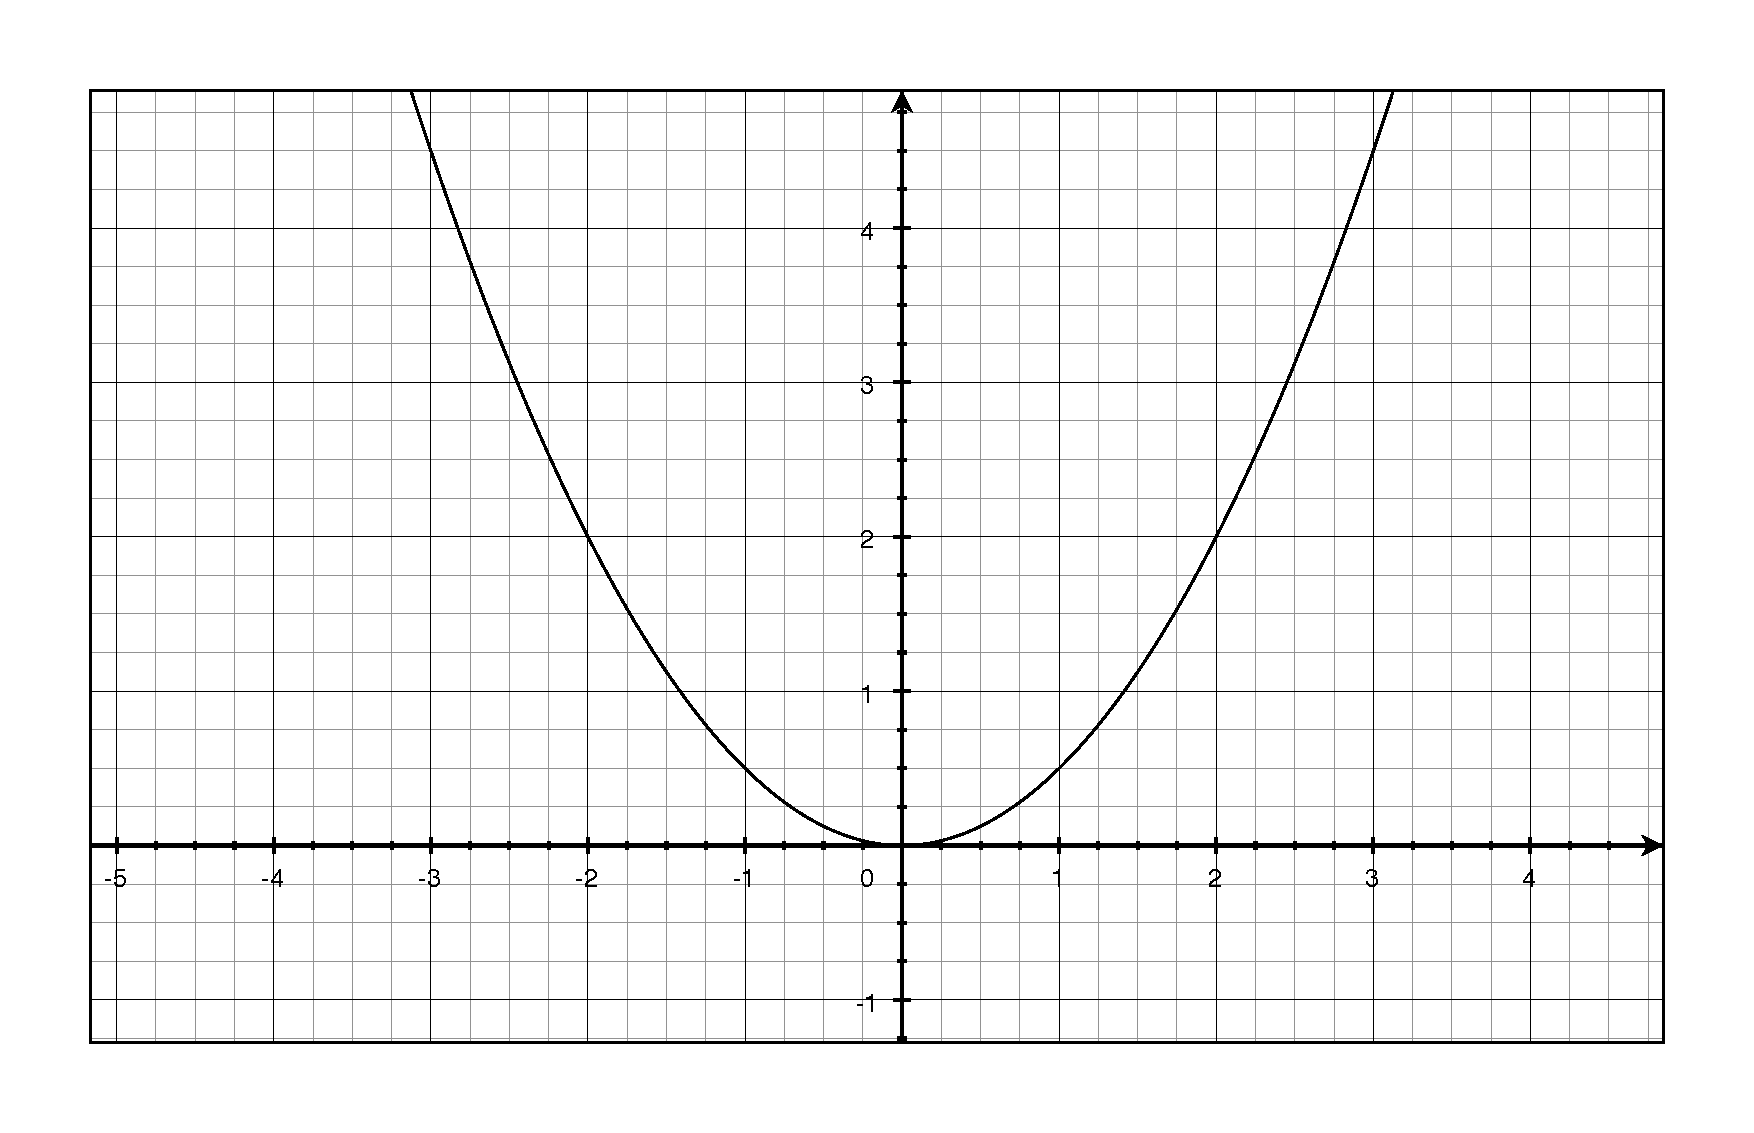
\includegraphics[scale=.3]{question11.eps}
  \caption*{Question 11}
\end{figure}

\item[12]
\begin{tabular}{ccc}
\toprule
vertex & focus & directrix \\
\midrule
  $(0, 0)$ & $\left(0, -\dfrac{1}{8} \right)$ & $y = \dfrac{1}{8}$ \\
\bottomrule
\end{tabular}

\begin{figure}[H]
  \centering
  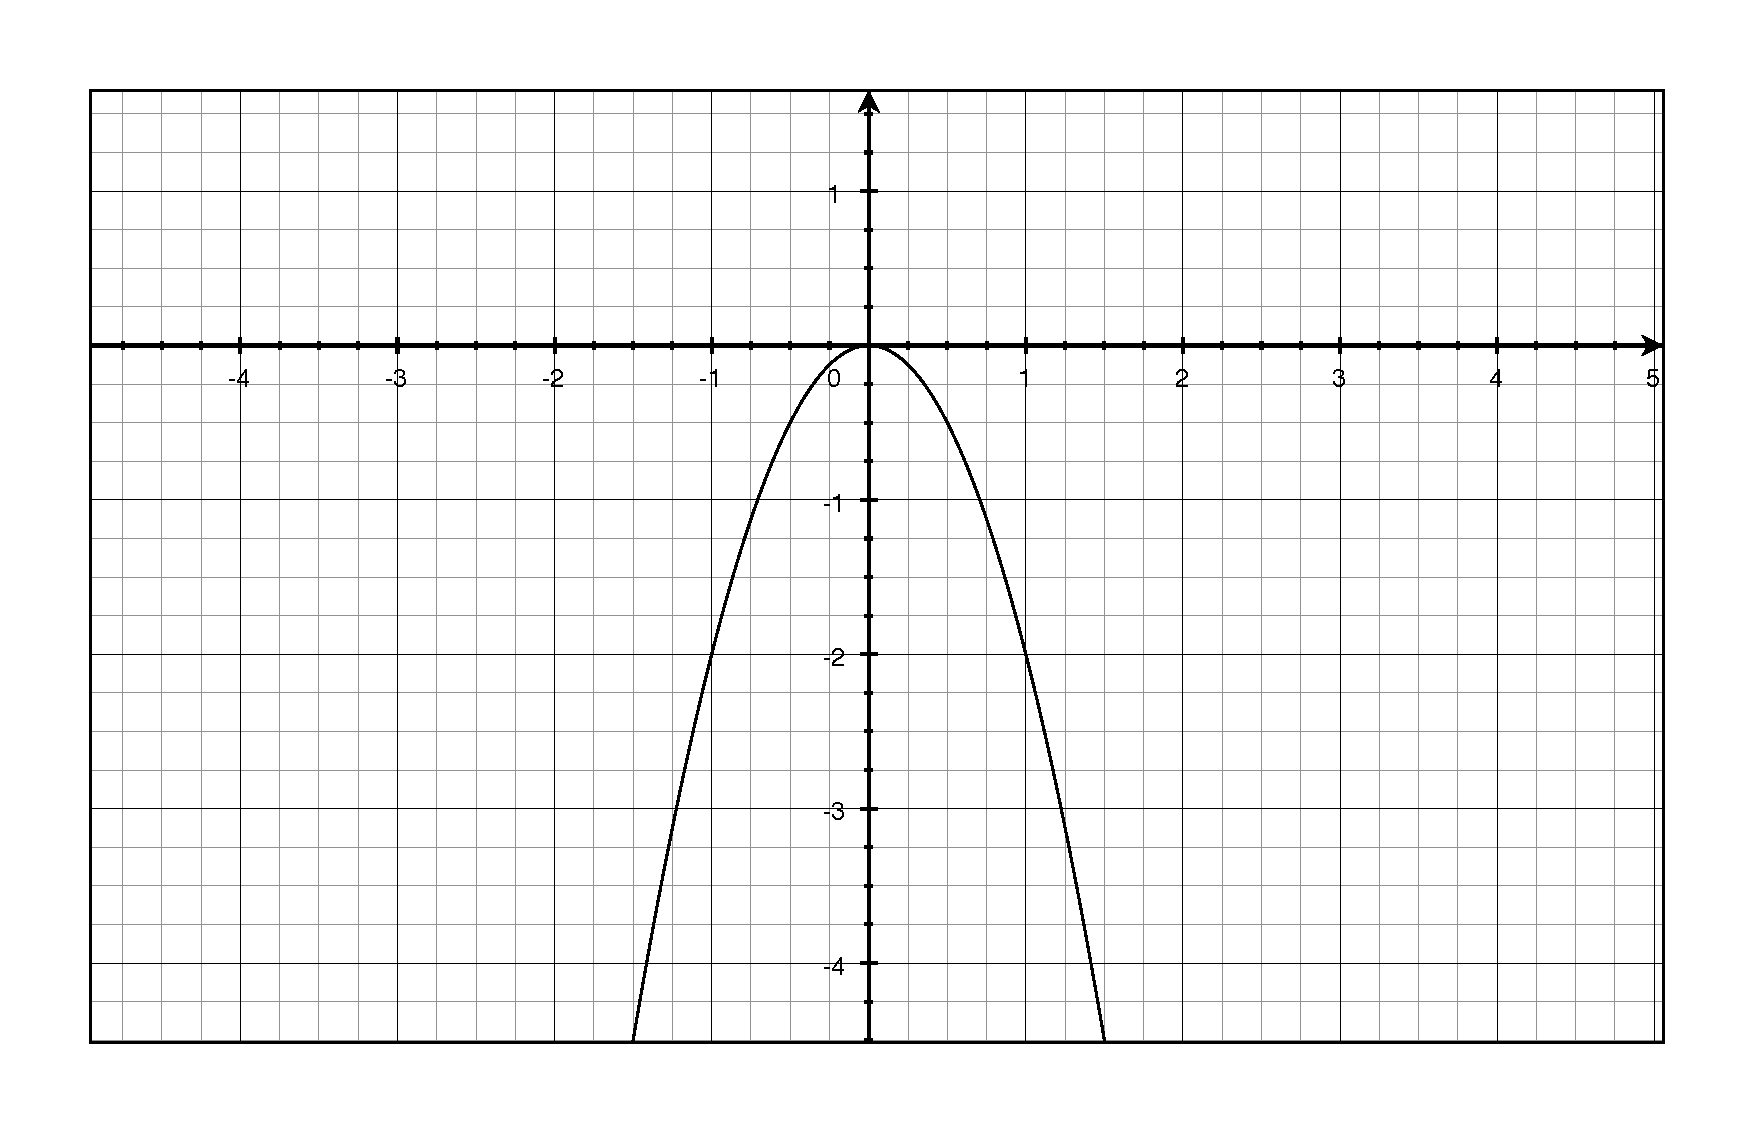
\includegraphics[scale=.3]{question12.eps}
  \caption*{Question 12}
\end{figure}

\item[17]
\begin{tabular}{ccc}
\toprule
vertex & focus & directrix \\
\midrule
  $(1, -2)$ & $\left(1, -4 \right)$ & $y = 0$ \\
\bottomrule
\end{tabular}

\begin{figure}[H]
  \centering
  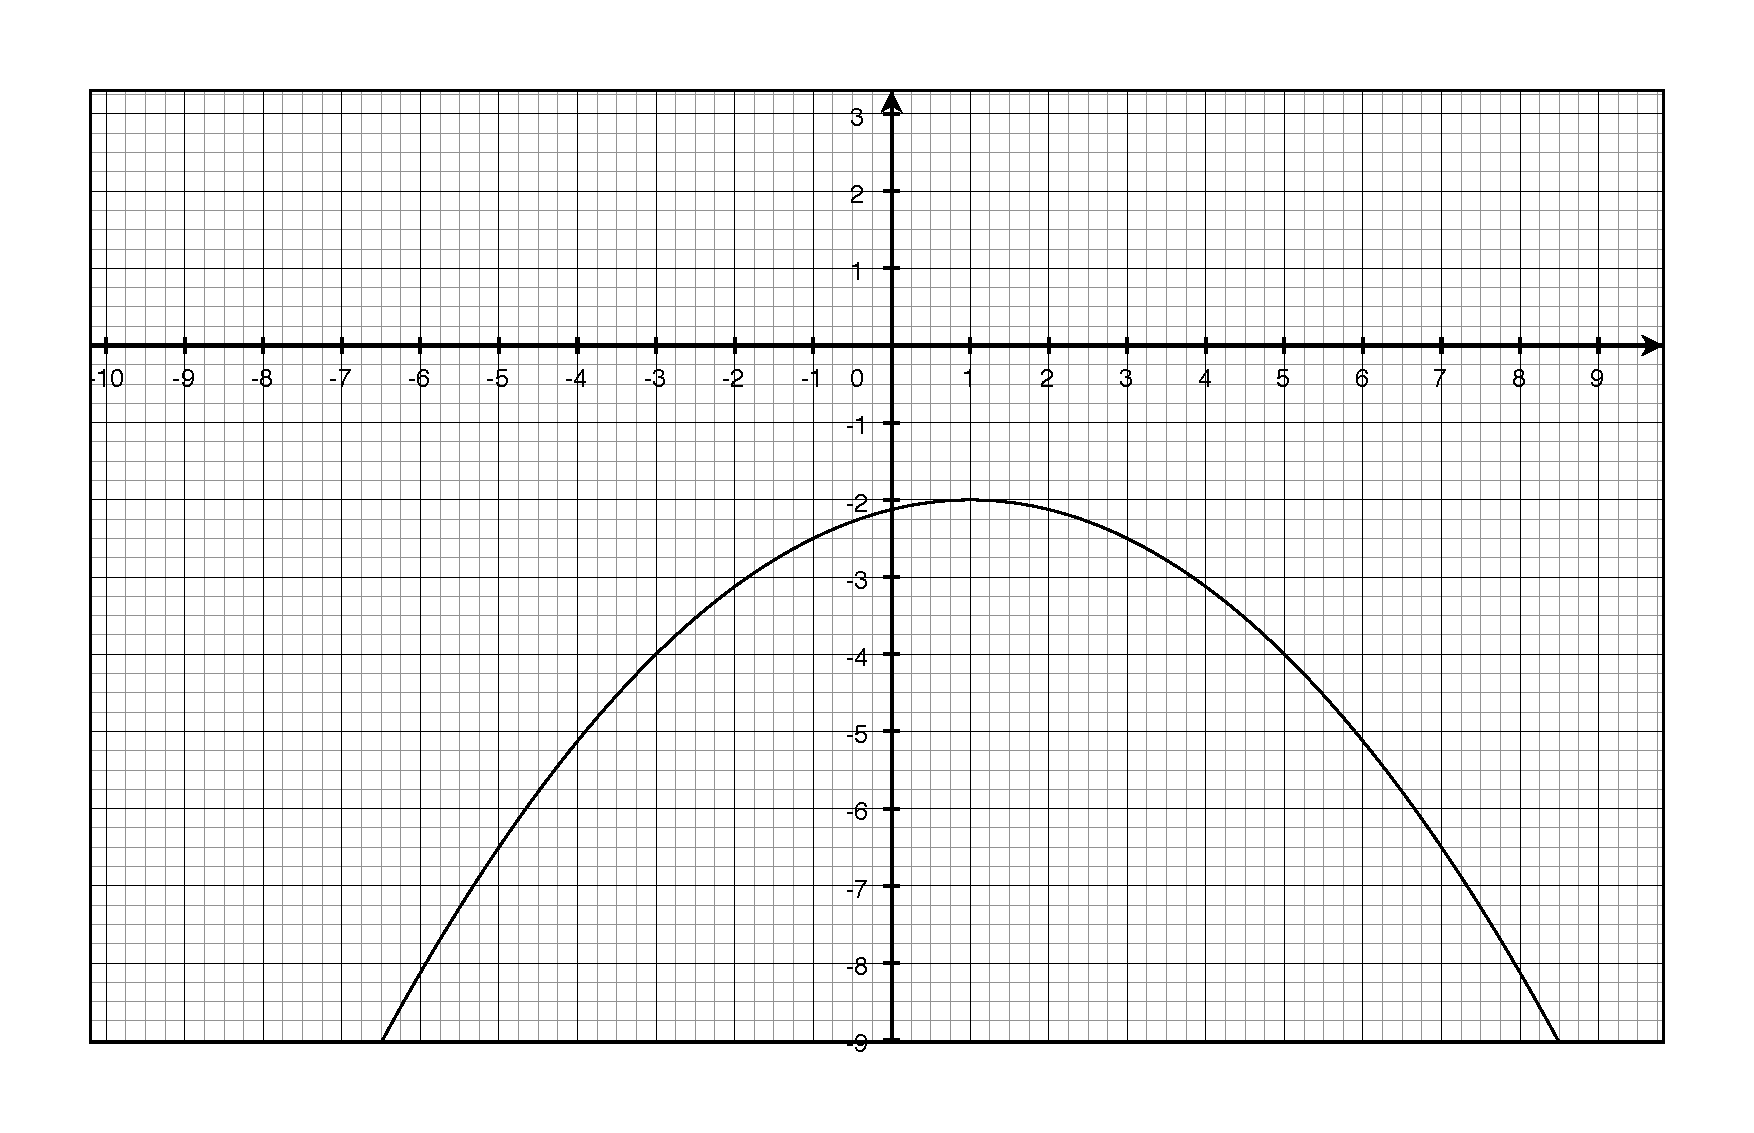
\includegraphics[scale=.3]{question17.eps}
  \caption*{Question 17}
\end{figure}

\item[18]
\begin{tabular}{ccc}
\toprule
vertex & focus & directrix \\
\midrule
  $(-5, 1)$ & $\left(-5, \dfrac{3}{4} \right)$ & $y = \dfrac{5}{4}$ \\
\bottomrule
\end{tabular}

\begin{figure}[H]
  \centering
  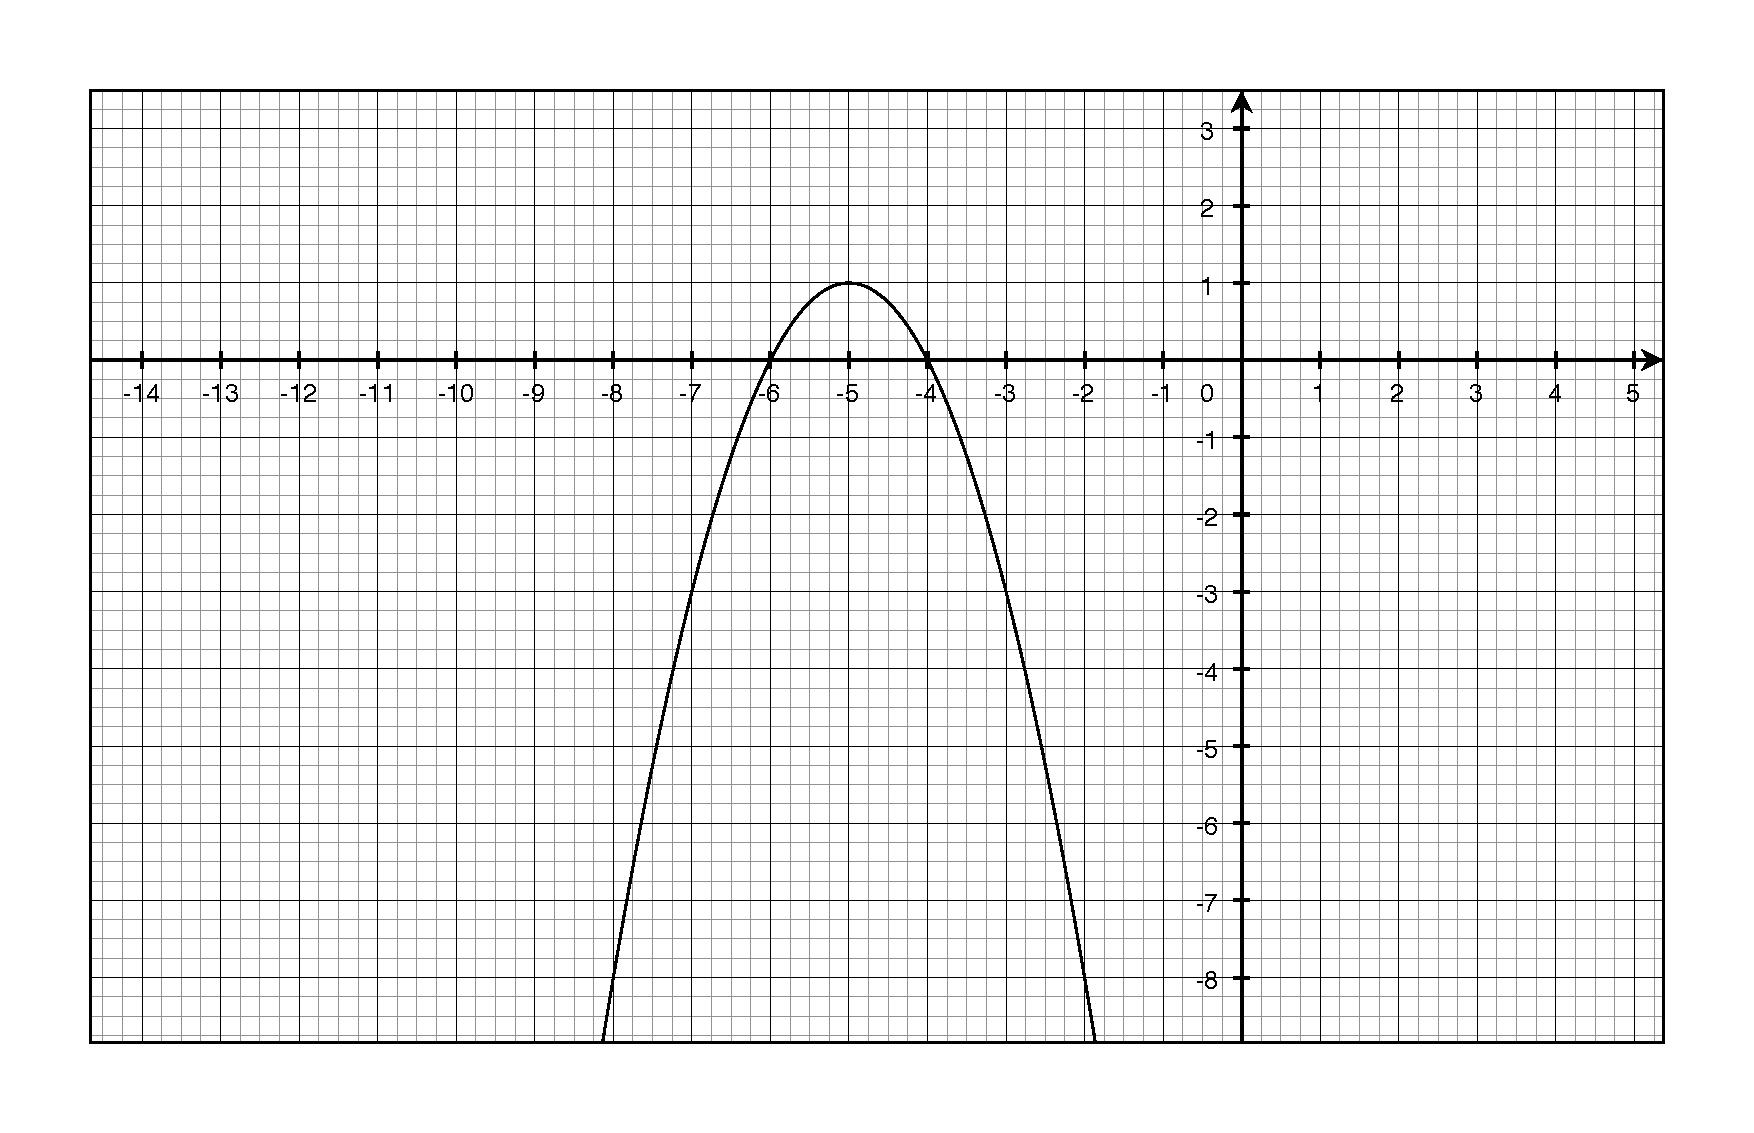
\includegraphics[scale=.3]{question18.eps}
  \caption*{Question 18}
\end{figure}

\item[23]
\begin{tabular}{ccc}
\toprule
vertex & focus & directrix \\
\midrule
  $(-2, -3)$ & $\left(-4, -3 \right)$ & $x = 0$ \\
\bottomrule
\end{tabular}

\begin{figure}[H]
  \centering
  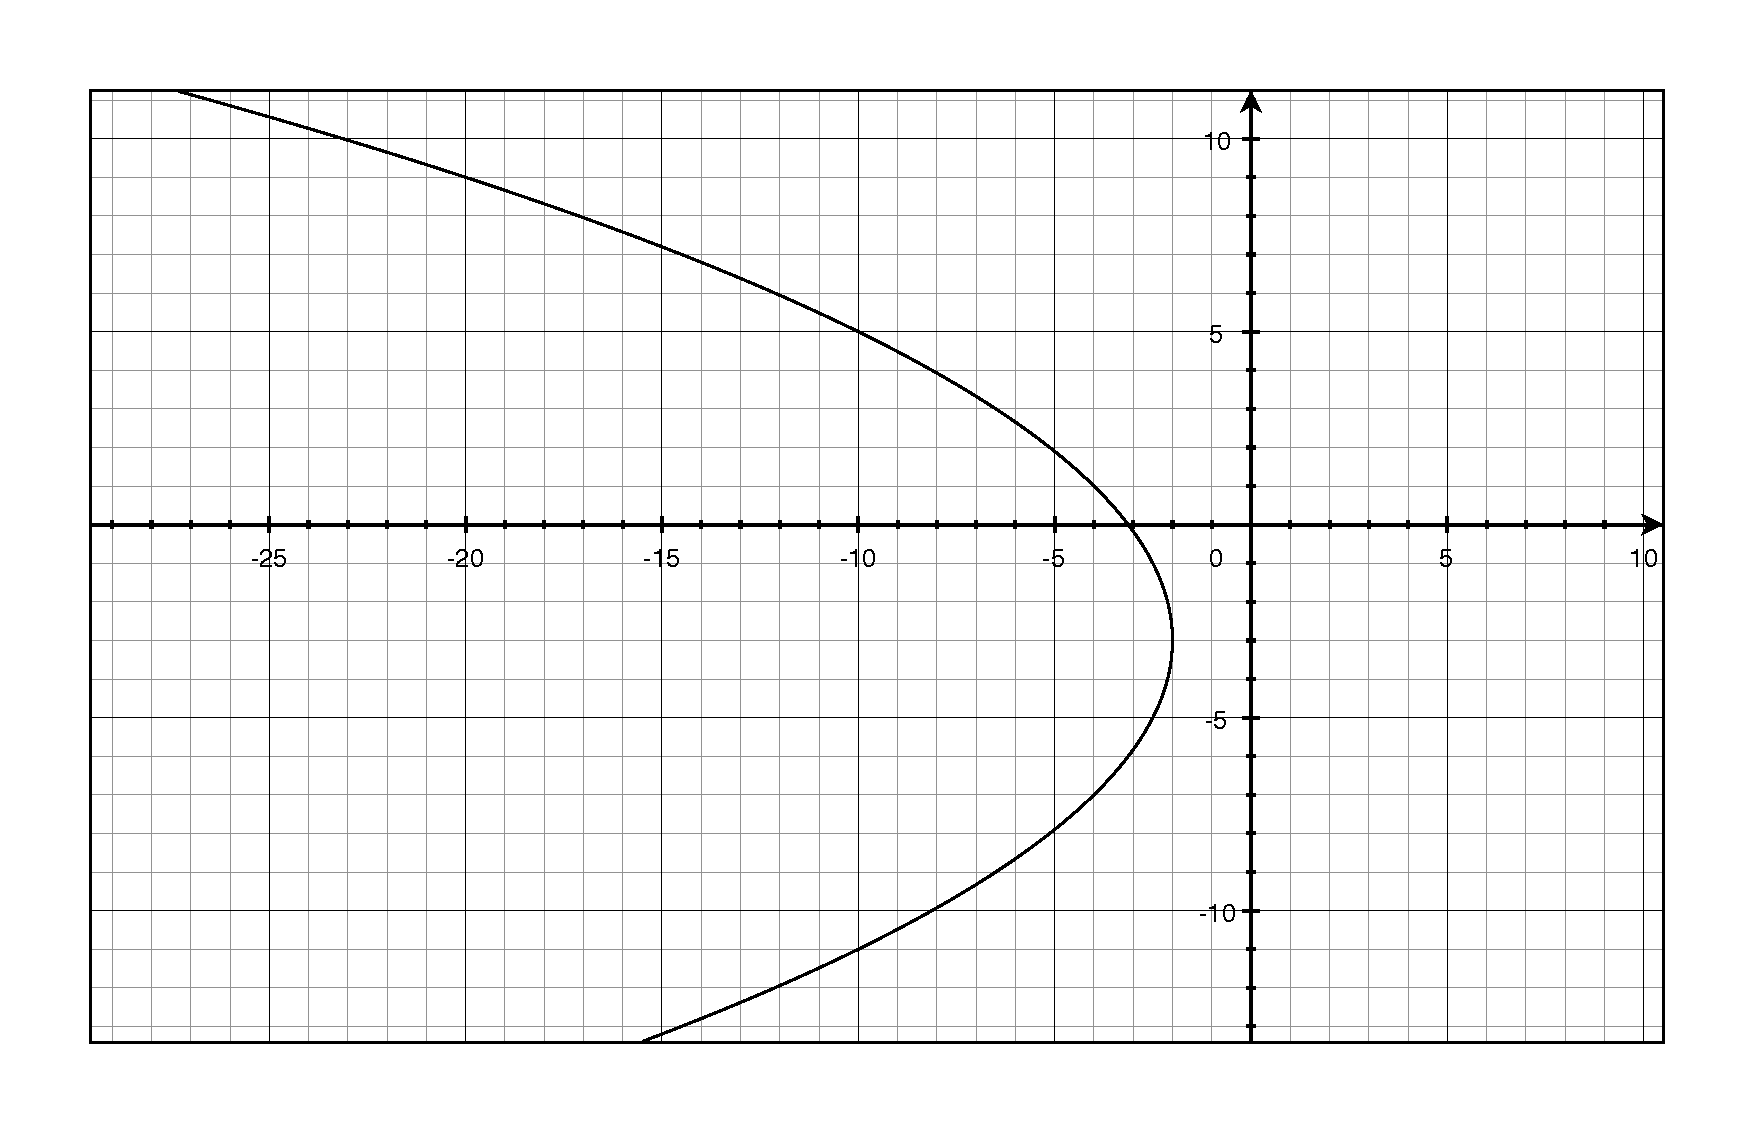
\includegraphics[scale=.3]{question23.eps}
  \caption*{Question 23}
\end{figure}

\item[24]
\begin{tabular}{ccc}
\toprule
vertex & focus & directrix \\
\midrule
  $(-1, 2)$ & $\left(0, 2 \right)$ & $x = -2$ \\
\bottomrule
\end{tabular}

\begin{figure}[H]
  \centering
  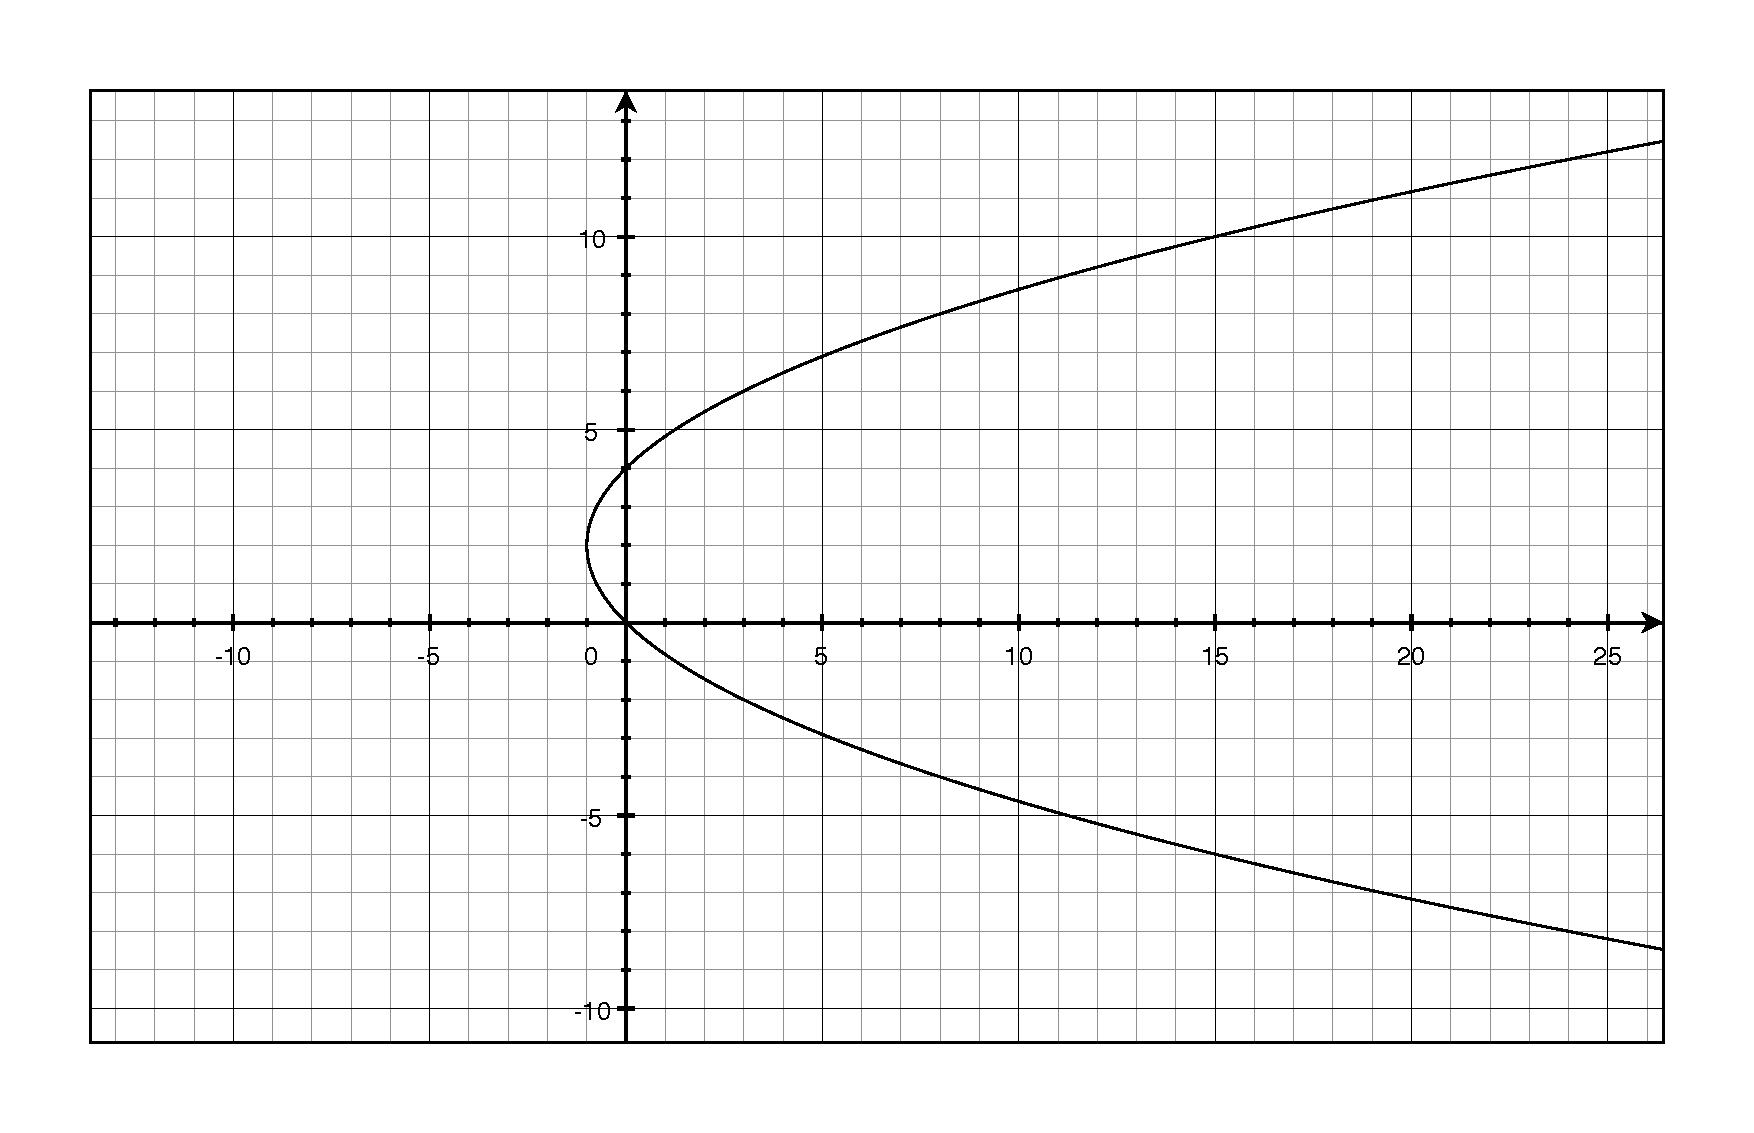
\includegraphics[scale=.3]{question24.eps}
  \caption*{Question 24}
\end{figure}

\item[31]
\begin{align*}
  x^2 &= 4 py \\
  9 &= 24 p \\
  p &= \frac{3}{8} \\
\end{align*}

So the equation is:
\[
  x^2 = \frac{3}{2} y
\]

\item[34]
focus: $(2, 0)$, $p = 2$

\[
  x^2 = 8y
\]

\item[37]
directrix: $y = -1$, $p = 1$

\[
  x^2 = 4y
\]

\item[47]
vertex: $(5, 2)$, focus: $(3, 2)$, $p = 2$

\[
(y-2)^2 = -8(x-5)
\]

\item[50]
vertex: $(-2, 1)$, directrix: $x=1$, $p = 3$

\[
  (y-1)^2 = -12(x+2)
\]

\item[61]
$p = 4.5$

$x^2 = 18y$ or $y = \dfrac{x^2}{18}$


\item[68]
false.  This would mean that $p=0$ which would make the graph a line instead of a parabola.

\item[69]
true

\end{description}


\else

\vspace{4 in}

\begin{em}
Whatever you do may seem insignificant to you, but it is most important that you do it. 
\end{em}

\vspace{.2 cm}
\hspace{1.5 cm} --Mohandas Gandhi 

\fi

\end{document}

